\section{System Architecture}
\label{sec:architecture}

Introductory paragraph explaining the system architecture. Explain that our
approach is to make PBS a shim layer on top of existing server code. Latency
measurements etc.

\begin{figure}
\centering
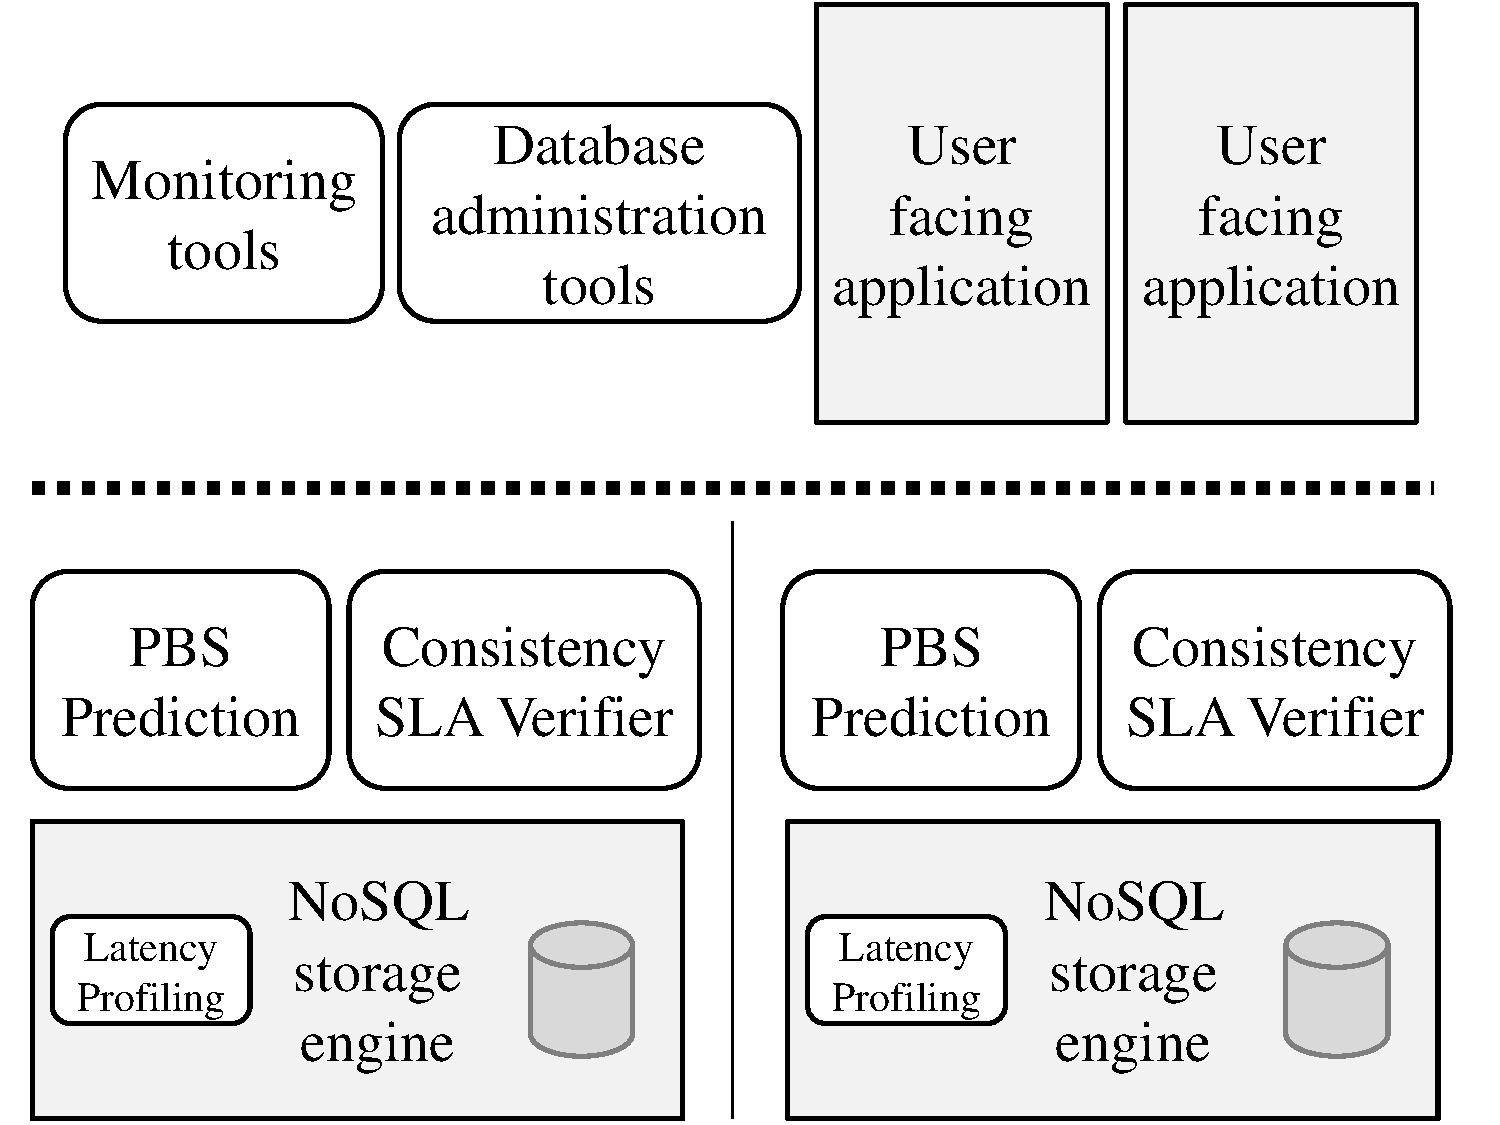
\includegraphics[width=.90\columnwidth]{figs/pbs-sys-arch.pdf}
\caption{Diagram showing how PBS metrics can be integrated into an existing
NoSQL datastore. The PBS prediction module and Consistency SLA verifier drive
the metrics used the monitoring framework.}
\label{fig:pbs-sys-arch}
\end{figure}

Walk through the system diagram - Explain what each component does. In
particular explain how the latency collector feeds into the PBS prediciton
module and how the Monte-Carlo simulation can be run using this data.

Talk about how the simulation can be triggered by either the database
administration tool or the Consistency SLA verifier module. The consistency sla
verifier accepts SLA specifications from clients and periodically triggers the
prediction module - This module also completes the loop and adjusts the value of
N,R and W until the consistency SLA is met.

Finally talk about how the database administration tool can also trigger the pbs
prediction. Explain how this works with respect to nodetool and the flexibility
they have with respect to the query inteface.

Last talk a little bit about the monitoring tools and how one can export the PBS
metrics in a time series format and alert the users if some trigger has not been
meet for the given time period.

Cassandra implementation details- this can either be meshed into each
component's description or it can be enumerated separately
